\documentclass[../main.tex]{subfiles}

\begin{document}

As mentioned in Chapter \ref{chap:implementation}, the approach to tackle the \gls{ctf} of the experimental images consists in correcting them with a Wiener filter. The issue of this approach is that not all frequencies can be recovered due to bad \gls{snr} or zero gain at the \gls{ctf}. Therefore, comparing those frequencies with the reference image may induce an artificial error. The aim of this section is to asses how this phenomenon affects the alignment accuracy.

To do so, several experiments will be carried out. Firstly, simulated images will be aligned with no \gls{ctf} being applied to them (only noise). Obviously, experimental images can not be evaluated without \gls{ctf}, as this is an artefact of the microscope. In any case, this experiment will be useful to observe the accuracy loss that can be attributed to the presence of the \gls{ctf}. Moreover, the ground truth alignment parameters of the simulated images are known. Therefore, once the \gls{ctf} has been applied to them, a reconstruction with these images is attempted. This gives an insight on the maximum achievable resolution with the simulated set of images. 

In the second trial, experimental images will be clustered by their \glspl{ctf}, so that the \gls{ctf} can be assumed to be constant across all images of a given group. This can not be easily done with simulated images, as these do not originate from a micrograph. Thus, simulated images will be left out from this experiment. Once the particles have been clustered according to their \glspl{ctf}, each of these image groups can be aligned against a reference set filtered with the representative \gls{ctf} of that group. This approach, similar to the one followed by current refinement packages, will establish the baseline for the alignment accuracy comparison with \gls{ctf}. 

Lastly, the \gls{ctf} will be corrected with a Wiener filter, both for experimental and simulated images. Then, these images will be aligned against a clean set of reference images. This will give an insight about the alignment quality degradation induced by aligning with Wiener corrected experimental images. 

Earlier, it was stated that most of the alignment information is contained below the resolution of $8\si{\angstrom}$. However, this alignment method targets the initial cycles of the refinement loop, where the reference volume has much less resolution. Therefore, these experiments will be carried out with a resolution limit of $15\si{\angstrom}$, so that the algorithm is evaluated on its operational range. At this resolution, typical \glspl{ctf} have one or two zero crossings. To ensure that the alignment errors can be attributed to the usage of the presence of the \gls{ctf} and the Wiener filter, no vector compression techniques will be used in these tests.

The tests have proved that using a Wiener filter to correct the \gls{ctf} of the images does not pose a significant penalty respect to applying the \gls{ctf} to the reference images. While it may introduce notable errors in certain simulated datasets (EMPIAR-10256 and EMPIAR-10391), the baseline for simulated datasets were images without \gls{ctf}. As a result, these errors can not be only attributed to the \gls{ctf} correction method but also the presence of the \gls{ctf} itself. Indeed, the experimental images were assessed against the conventional \gls{ctf} correction method. Figures \ref{fig:5:ctf_angle_accuracy} and \ref{fig:5:ctf_shift_accuracy} show that for experimental datasets, the angle and shift assignment error increase induced by the Wiener \gls{ctf} correction is around $8 \si{\percent}$.

It can be noted that the angular assignment error for EMPIAR-10256 is considerably higher than the rest. This is because the calumnium bound to the TPRV5 protein exhibits mismatched symmetry. This means that there is a predominant symmetry which is not followed across all the regions of the protein. In this case, the TPRV5 protein has C4 symmetry but the calumnium is bound off-centred, breaking ensemble's symmetry. As a consequence, it is not easy to distinguish between symmetrical views of the TPRV5. This angular error will be a trend for the rest of the tests conducted with this dataset.

\begin{figure}[htbp]
    \centering
    \begin{subfigure}[b]{.8\textwidth}
         \centering
         \includegraphics[width=\linewidth]{results/ctf/simulated/angle error}
         \caption{Simulated images}
    \end{subfigure}\\
    \vspace{2em}
    \begin{subfigure}[b]{.8\textwidth}
         \centering
         \includegraphics[width=\linewidth]{results/ctf/experimental/angle error}
         \caption{Experimental images}
    \end{subfigure}
    \caption{Angle accuracy for different compression methods}
    \label{fig:5:ctf_angle_accuracy}
\end{figure}

\begin{figure}[htbp]
    \centering
    \begin{subfigure}[b]{.8\textwidth}
         \centering
         \includegraphics[width=\linewidth]{results/ctf/simulated/shift error}
         \caption{Simulated images}
    \end{subfigure}\\
    \vspace{2em}
    \begin{subfigure}[b]{.8\textwidth}
         \centering
         \includegraphics[width=\linewidth]{results/ctf/experimental/shift error}
         \caption{Experimental images}
    \end{subfigure}
    \caption{Shift accuracy for different compression methods}
    \label{fig:5:ctf_shift_accuracy}
\end{figure}

Regarding the reconstruction resolution of the particles, the results are even better than the previous ones. Comparatively, the resolution degradation associated to the introduction of the Wiener filter is around $3 \si{\percent}$ for experimental images. Furthermore, the high angle assignment errors of the EMPIAR-10256 do not correlate with a loss in resolution, as the resolution obtained for this dataset is similar to the one obtained for the rest. This is because the incorrectly assigned views are still highly compatible with the reconstructed volume.

\begin{figure}[htbp]
    \centering
    \begin{subfigure}[b]{.8\textwidth}
         \centering
         \includegraphics[width=\linewidth]{results/ctf/simulated/resolution}
         \caption{Simulated images}
    \end{subfigure}\\
    \vspace{2em}
    \begin{subfigure}[b]{.8\textwidth}
         \centering
         \includegraphics[width=\linewidth]{results/ctf/experimental/resolution}
         \caption{Experimental images}
    \end{subfigure}
    \caption{Reconstruction resolution for different compression methods}
    \label{fig:5:ctf_resolution}
\end{figure}

\end{document}